\Chapter{Koncepció}
% TODO: Le kellene írni az OBJ formátumról a fontosabb dolgokat!
\Section{OBJ fájlformátum}

Az OBJ fájlformátumot elsőnek a Wavefront Technologies kezdte kifejleszteni az 1980-as években az Advanced Visualizer animációs csomagjához. Ez a formátum egy olyan karakteres fájlformátum, ami utat enged geometriai objektumok leírásának egy aránylag egyszerű és egységes formában. \\
Magát a formátumot ott logikus használni, ahol egyszerű modelleket jelenítünk meg és ezeket nem akarjuk animálni. Például egy olyan egyszerű autó szimulátoros játéknál, ahol maga az autó geometriáját tekintve nem változik maximum a pozíciója és az orientációja, ezeket a transzformációs mátrix állításával egyszerűen megadhatjuk, így nincs szükség a modell animálására.\\
Wavefront formátumbemutatása egy egyszerű példával, ez a példa egy szimpla négyszöget definiál:\\

\begin{cpp} 
# ez egy comment

v 0.0 0.0 0.0
v 1.0 0.0 0.0
v 1.0 1.0 0.0
v 0.0 1.0 0.0

vt 0.0 0.0
vt 1.0 0.0
vt 1.0 1.0
vt 0.0 1.0

vn 1.0 0.0 0.0 

f 1/1/1 2/2/1 3/3/1 4/4/1
\end{cpp}

A fájl először felsorolja a csúcspontokat \textbf{v} (vertex), utána a textúra pontokat \textbf{vt} (vertex texture) és a normálvektorokat \textbf{vn} (vertex normal) utána  az \textbf{f} (face) kulcsszóval egymáshoz rendeli ezeket. A lap utasításban például a lapot négy csúcsponttal adtuk meg (ez egy négyszög), és / jellel elválasztva minden csúcshoz közöltük a csúcspont, a textúra pont és a normálvektor sorsszámát. \newpage

\noindent A következő példa egy kockát fog definiálni:\\
\begin{cpp} 
v 1.0 1.0 0.0
v 1.0 1.0 -1.0
v 0.0 1.0 -1.0
v 0.0 1.0 0.0
v 1.0 0.0 -1.0
v 0.0 0.0 -1.0
v 1.0 0.0 0.0
v 0.0 0.0 0.0

vt 1.0 0.0
vt 1.0 1.0
vt 0.0 1.0
vt 0.0 0.0

vn 0.0 1.0 0.0
vn 0.0 0.0 -1.0
vn 0.0 -1.0 -0.0
vn 1.0 -0.0 0.0
vn -1.0 0.0 0.0
vn 0.0 -0.0 1.0

f 1/1/1 2/2/1 3/3/1 4/4/1
f 2/3/2 5/4/2 6/1/2 3/2/2
f 5/1/3 7/2/3 8/3/3 6/4/3
f 5/1/4 2/2/4 1/3/4 7/4/4
f 8/1/5 4/2/5 3/3/5 6/4/5
f 7/1/6 1/2/6 4/3/6 8/4/6
\end{cpp}
\noindent A kocka megjelenítése:

\begin{figure}[h]
\centering

\includegraphics[scale=0.23]{images/cube_notexture.png}
\caption{Kocka.}
\end{figure}

A négyzethez hasonlóan felsorolja a csúcspontokat \textbf{v} (vertex), de azzal ellentétben itt már nem 4 csúcspont található, hanem 8 mivel a kocka összes csúcspontját definiálni kell a formátumnak. A \textbf{vn} (vertex normal), illetve a \textbf{f} (face) szám is megváltozik a kocka lapjainak számával arányosan.\newline


\noindent Most következzen pár gyakran előforduló face definíció:\newline

\noindent Csak vertexekből áll a felület.
\begin{cpp} 
f v1 v2 v3 v4 ...
\end{cpp}
Minden vertexhez hozzá van rendelve egy textúra koordináta is.
\begin{cpp} 
f v1/vt1 v2/vt2 v3/vt3 ...
\end{cpp}
Minden vertex tartalmaz textúra koordinátát és normál vektort.
\begin{cpp} 
f v1/vt1/vn1 v2/vt2/vn2 v3/vt3/vn3 ...
\end{cpp}
A vertexekhez csak a felületi normális lett hozzárendelve, a textúra pont opcionális.
\begin{cpp} 
f v1/ /vn1 v2/ /vn2 v3/ /vn3 ...
\end{cpp}
Összefoglalva, az OBJ formális nyelv kulcsszavakból (<\textbf{v}>, <\textbf{vt}>, <\textbf{vn}>, <\textbf{f}>), speciális karakterekből (<\textbf{/}>) és számokból (<\textbf{Float}>, <\textbf{Integer}>) épül fel. Az OBJ nyelvtanát következő szabályokkal adhatjuk meg:\\

\noindent(OBJFile) = {(Vertex)}+{(VertexTexture)}+{(VertexNormal)}+{(Face)}\\
(Vertex) = (v)+(Float)+(Float)+(Float)\\
(VertexTexture) = (vt)+(Float)+(Float)+[0]\\
(VertexNormal) = (vn)+(Float)+(Float)+(Float)\\
(Face) = (f)+{(VertexOfFace)}\\
(VertexOfFace) = (Integer)+[(/)+[(Integer)]+[(/)+[(Integer)]]]\\

A szögletes zárójel [ ] az opcionalitás jele, azaz a benne foglalt fogalom egyszer vagy egyszer sem jelenik meg. A teljes OBJ formátum nagyon komplex, sok olyan eszköz van benne, ami egy „egyszerű” objektum modellezéséhez feleslegesnek mondható.Az OBJ formátum a 3D színtérben elhelyezkedő objektumok geometriáját írja le csupán. Ezen felül szükség van még az anyagjellemzőkre is a képszintézis során.\newpage

\Section{Anyagjellemzők}

A különböző anyagokat (felületeket) a fizikai tulajdonságaikkal írjuk le. Ilyen tulajdonság például a fényáteresztő képesség,fényvisszaverő képesség, törésmutató, szín stb. \newline

\noindent Itt több lehetőség közül választhatunk:\newline

Az egyik lehetőség hogy ezeket a tulajdonságokat az MTL (Material Template Library) tartalmazza, ami hasonlóan az OBJ fromátumhoz szintén szöveges és az OBJ fájl tartalmazza a hivatkozást a megfelelő MTL fájlra:
\begin{cpp} 
mtllib filename.mtl
\end{cpp}
Ebben az esetben az \textbf{mtllib} jelzi az MTL fájlt, majd a  \textsl{fájlnév} következik.\newline

A másik lehetőség, hogy ezeket a tulajdonságokat a megjelenítőnk segítségével állítjuk be a kívánt értékre.\newline

\noindent \textbf{Ambient:}

Az anyag \textsl{ambient} (MTL fájlban \textbf{Ka}) – a környezettől független színét írja le. Az ambient tulajdonság úgy viselkedik mint a foszforeszkálás, tehát ha nem éri fény a testet, akkor is ilyen lesz a színe.

\begin{figure}[h]
\centering
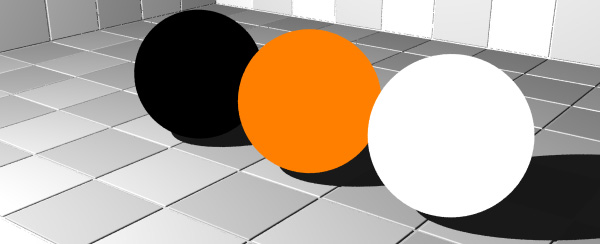
\includegraphics[scale=0.5]{images/ambient.jpg}
\caption{Ambient.}
\end{figure}
Fontos megjegyezni, hogy az \textsl{ambient} tulajdonság nem fényforrás, tehát attól, hogy egy testnek \textsl{ambient} színe van, nem fogja megvilágítani a mellette álló másik testet. Az értékét RGB-ben adjuk meg, a szokott módon.
\newpage
\noindent \textbf{Diffuse:}

Az anyag \textsl{diffuse} "szórt" (MTL fájlban \textbf{Kd}) – alap színét írja le. Ez a legegyszerűbb, lényegében egy test színét határozza meg. Pontosítva a dolgot, azt mondhatjuk, hogy a diffuse tulajdonság határozza meg, hogy a felület, a rá eső fény mely komponenseit nyeli el.

\begin{figure}[h]
\centering
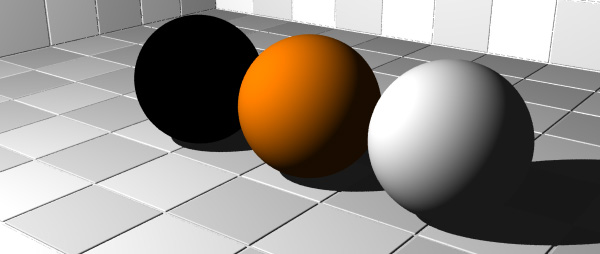
\includegraphics[scale=0.5]{images/diffuse.jpg}
\caption{Diffuse.}
\end{figure}
Ahol nem éri fény a testet, ott nem fog érvényesülni diffúz hatása, ott tehát fekete lesz a test (árnyék). A diffúz értékét RGB -ben kell megadni.\newline

\noindent \textbf{Specular:}

Az anyag \textsl{specular} (MTL fájlban \textbf{Ks})  - színét határozza meg, ami nem más, mint tükröződés. Ha 1 1 1 -es értéket adunk neki, akkor tökéletes tükörként viselkedik (vagyis minden fényt visszaver, ami rá esik), ha 0 0 0 az értéke, akkor pedig egyáltalán nem tükröződik.

\begin{figure}[h]
\centering
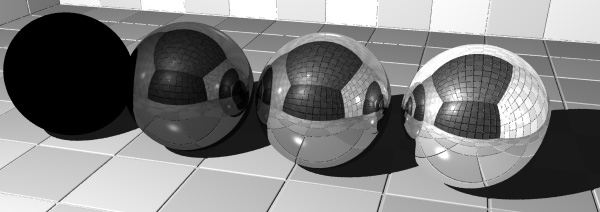
\includegraphics[scale=0.5]{images/specular.jpg}
\caption{Specular.}
\end{figure}

\noindent \textbf{Emissive:}

Az \textsl{ambient} , \textsl{diffuse}, \textsl{specular} komponensek mellet van egy negyedik is, mégpedig az \textsl{emissive} (MTL fájlban \textbf{Ke})összetevő. Ez egy olyan komponens, mely az előbbi háromhoz adódik hozzá, a felület világosabb lesz általa, mintha saját maga bocsátaná ki a saját fényét.\newline

\noindent \textbf{Shininess:}

A felületek általában nem csak tükörszerűen viselkednek, hanem van "saját fényük", "csillogásuk" is. Az \textsl{shininess} (MTL fájlban \textbf{Ns}) ezt hivatott ábrázolni. A spekuláris fénysávok élességét határozza meg (minél nagyobb, annál élesebb).

\begin{figure}[h]
\centering
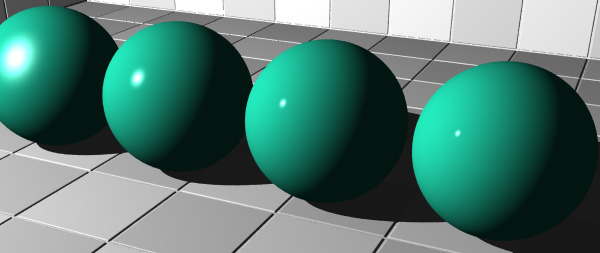
\includegraphics[scale=0.5]{images/shine.jpg}
\caption{Shine.}
\end{figure}
\newpage
\Section{Textúrák}

%\Section{Obj elemző szoftverek}
%\Section{Obj Bickbucket}
%\Section{Obj Bickbucket teszt}